\lstset{style=pythoninlinestyle}

\section{СИСТЕМНОЕ ПРОЕКТИРОВАНИЕ}
\label{sec:sys}

\subsection{Постановка задачи на разработку программного средства}
\label{sub:sys:1}

В классической постановке, пусть задано $k$ входных и выходных   переменных (для примера - три входных переменных $x$, $y$, $z$ и одна выходная переменная $w$). Пусть определены лингвистические значения этих переменных $A$,$B$,$C$,$D$,$E$,$F$ для $n$ правил (для примера $n=3$).  Типичный вариант представления логического вывода, с этапами фаззификации,  агрегирования и дефаззификации показан на рис. 2.1.

\begin{figure}[ht]
  \centering
  \fbox{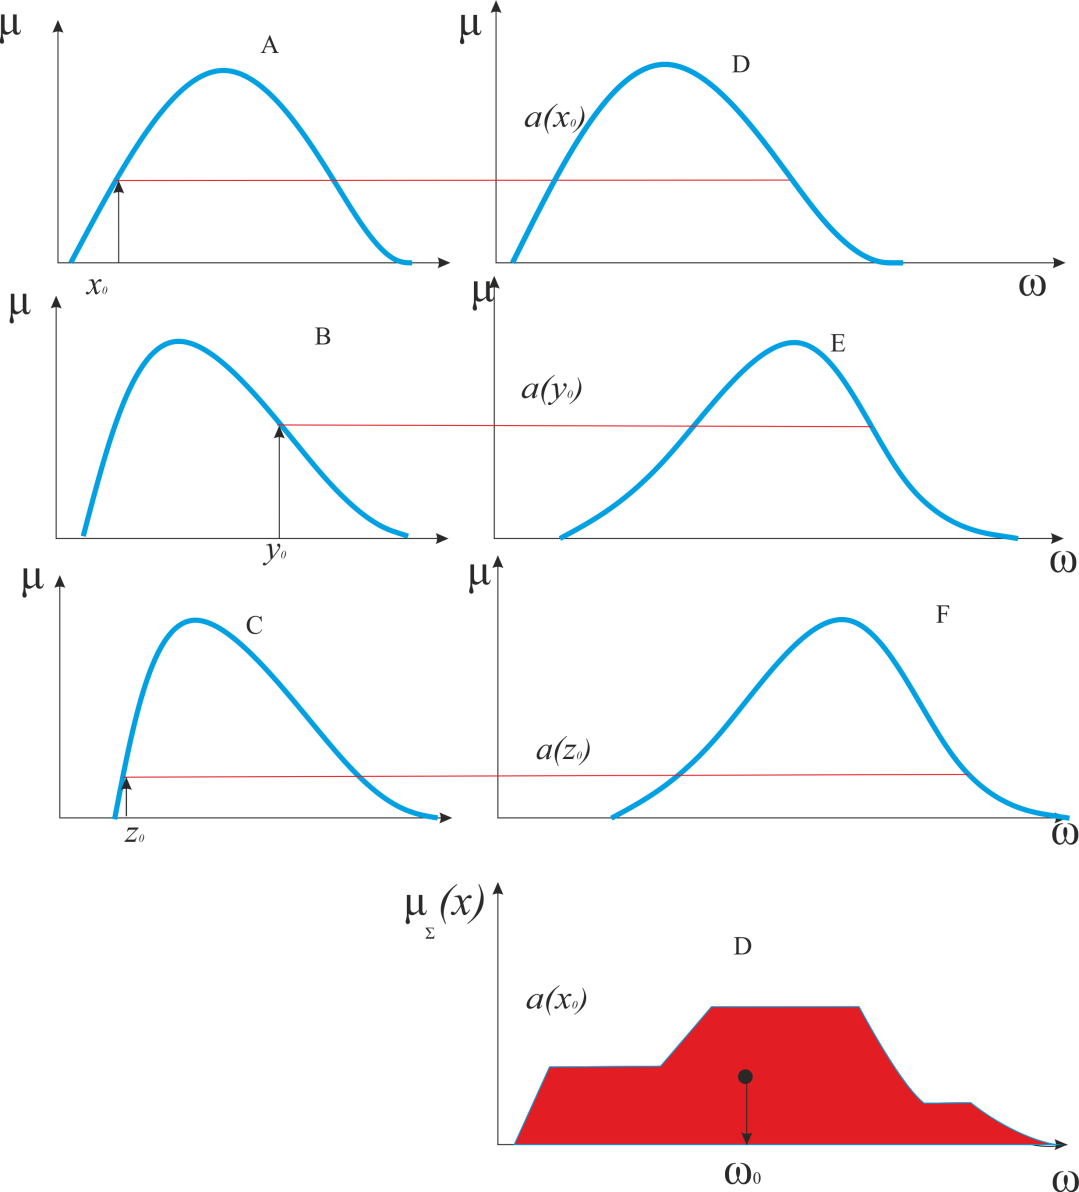
\includegraphics[scale=0.3]{2-1.png}}
  \caption{Вариант представления логического вывода, с этапами фаззификации,  агрегирования и дефаззификации }
  \label{fig:sys:1:1}
\end{figure}

Точные исходные данные с датчиков, контролирующих управляющий процесс, переводятся в значения лингвистических переменных в специальном блоке фаззификатора. Далее реализуются процедуры нечеткого вывода на множестве продукционных правил, составляющих базу знаний системы управления, в результате чего формируются выходные лингвистические значения, которые переводятся в точные значения результатов вычислений в блоке дефаззификатора. На выходе последнего формируются управляющие воздействия на исполнительные механизмы. Эта концептуальная схема лежит в основе нечеткого контроллера. И выполнение работы каждого блока нечеткого контроллера требует достаточного выделения ресурсов и времени на выполнение задач. [4]

Для отладки нечеткого контроллера могут применяться натурные эксперименты, но их проведение сопряжено со значительными временными и финансовыми, сложностью доступа к оборудованию, формированию полигона, погодных условия и так далее. Логичным решением этой проблемы представляется программное моделирование экспериментов, что позволяет значительно упростить, ускорить и удешевить настройку и отладку нечетких контроллеров. Многие реализации нечетких контроллеров основаны на классических алгоритмах, поэтому разрабатываемое программное средство должно содержать гибко настраиваемую реализацию одного из классических алгоритмов нечеткого вывода, на основе которого экспериментатор сможет реализовать собственный нечеткий контроллер. Поскольку нечеткие контроллеры – это активно развивающееся направление, разрабатываемое программное средство должно позволять с минимальными трудозатратами подключать реализованные экспериментатором алгоритмы нечетких контроллеров. Визуализация результатов эксперимента в виде графиков и диаграмм обычно требует установки, настройки и освоение стороннего программного обеспечения, поэтому разрабатываемое программное средство должно позволять отображать результаты экспериментов. Настройка алгоритмов нечеткого вывода является трудоемкой, поэтому программное средство должно иметь средства автоматизации обучения нечетких контроллеров.

Таким образом можно сформулировать требования к программному средству для отладки алгоритмов нечеткого управления мобильными роботами:

\begin{itemize}
  \item содержать в себе готовую, настраиваемую модель нечеткого контроллера на базе классического алгоритма нечеткого вывода;
  \item иметь возможность подключения реализованных экспериментатором моделей нечетких контроллеров;
  \item позволять гибко настраивать конфигурацию и характеристики моделируемого пути;
  \item иметь возможность визуализации, сравнения и сохранения полученных в результате эксперимента данных;
  \item иметь средства автоматизированной генерации лингвистических переменных, термов и правил нечетких алгоритмов;
  \item быть доступной для освоения в короткие сроки.
\end{itemize}

\subsection{Разработка обобщенной модели}
\label{sub:sys:2}

Обобщенная схема эксперимента представлена на чертеже ГУИР ГУИР.400201.322 ПД1. Опишем ее блоки.

\subsubsection{Ввод $S_0$, $V_0$}

В начале эксперимента в качестве исходных данных задаются начальная скорость $V_0$ и начальное расстояние до препятствия $S_0$.

\subsubsection{Расчет усилия }

В каждом кванте модельного времени производится расчет тормозного усилия. Расчет производится нечетким алгоритмом на основании текущей скорости, текущего расстояния до препятствия, заданных термов лингвистических переменных и базы правил. Последние получены в результате работы алгоритма настройки и обучения.

\subsubsection{ Моделирование замедления}

На основании расчетного усилия  замедления и характеристик моделируемого пути в данной точке рассчитывается значение отрицательного ускорения, которое будет действовать на платформу в текущий момент модельного времени.

\subsubsection{Расчет мгновенных $V'$, $S'$ для текущего модельного времени $T$}

На основании рассчитанного в п. 2.1.3 ускорения, а также расстояния и пути $S$ и $V$ для предыдущего кванта модельного времени, рассчитываются новые значения $V`$ и $S`$ для текущего модельного времени.

\subsubsection{ $S = 0$ или $V = 0$? }
Здесь выполняется проверка: если расстояние до препятствия равно нулю, либо мгновенная скорость равна нулю, эксперимент окончен, иначе повторения цикла. Действительно: если скорость равна нулю, то, очевидно, дальнейшее положение платформы не изменится, она успешно остановилась. Верно и другое: если расстояние до препятствия равно нулю, значит произошло столкновение.

\subsubsection{ Алгоритм настройки и обучения }

Области определения лингвистических переменных, функции принадлежности термов, а также правила задаются в результате работы алгоритма настройки и обучения. Проектируемое программное средство позволяет задавать вышеупомянутые переменные и правила в автоматизированном режиме на основе эталонных данных.

\subsection{Методика тестирования и отладки алгоритмов нечеткого управления; алгоритм настройки нечеткого контроллера}

Основной проблемой создания нечеткого регулятора является конструирование базы знаний, содержащей опыт и знания человека – оператора. Заполнение базы знаний может выполняться различными способами [9]:

\begin{enumerate}[label=\arabic*)]
  \item Оператор-эксперт управляет технологическим процессом, за которым <<наблюдает>> регулятор, запоминая все действия эксперта и заполняя свою базу знаний.
  \item Оператор-эксперт описывает свое действие при каждой наблюдаемой ситуации в виде продукции <<если..., то... >>, которые и будут образовывать базу знаний регулятора.
  \item Перед самоорганизующимся нечетким регулятором ставится цель обеспечить желаемую переходную характеристику проектируемой системы и одновременно сообщается некоторая информация о технологическом процессе (объекте управления). Регулятор самостоятельно (методом проб и ошибок) накапливает знания без эксперта.
\end{enumerate}

Кроме рассмотренной структуры возможны и более сложные, способные адаптировать к изменениям окружающей среды путем переключений на другие множества лингвистических значений, продукционные правила, базы знаний [10].

При реализации данного программного средства использовалась комбинация первого и второго подходов: на основании собранных данных в результате моделирования с применением <<наивного>> алгоритма, блок обучения нечеткого контроллера генерирует предварительный набор правил, которые затем донастраиваются оператором (экспертом).

\subsection{Структурная схема экспериментального программного обеспечения}
\label{sub:sys:4}

Изучив теоретические аспекты разрабатываемой системы и выработав список требований необходимых для разработки системы, разбиваем систему на функциональные блоки(модули). Такой подход позволяет изменять или заменять модули без изменения всей системы в целом.

В разрабатываемом приложении можно выделить следующие блоки:

\begin{itemize}
  \item блок пользовательского интерфейса;
  \item блок диспетчера приложения;
  \item блок обучения нечетких контроллеров;
  \item блок визуализации телеметрии;
  \item блок симуляции;
  \item блок физической модели;
  \item блок моделирования нечетких алгоритмов;
  \item блок сбора телеметрии.
\end{itemize}

Структурная схема, иллюстрирующая перечисленные блоки и связи между ними приведена на чертеже ГУИР.400201.322 С1.

Каждый модуль выполняет свою задачу. Чтобы система работала каждый модуль взаимодействует с другими модулями путем обмена данными, используя различные форматы и протоколы.

Рассмотрим функциональные блоки приложения.

\subsubsection{Блок пользовательского интерфейса}

Реализует интерфейс командной строки, Command Line Interface (CLI). Для профессионального научного ПО CLI имеет ряд преимуществ. Рассмотрим их ниже.

\textit{Масштабируемость}. Любой, кто достаточно хорошо разбирается в управлении cookie в Firefox, вероятно, столкнутся с <<проблемой 1001 cookies>>, где окна диалога управления файлами cookie появляются так быстро и в таких количествах, что кажется, что может пройти весь день, чтобы пройти через все их. В этом примере демонстрируется проблема Graphical User Interface (GUI) и других интерактивных интерфейсов: масштабируемость. Когда вы выполняете только одну, простое задание один раз, может показаться довольно простым просто щелкнуть пару кнопок интерфейса и перейти дальше. Когда внезапно возникает избыток таких задач, и все они требуют внимания пользователя (например, выбирать, какие cookie принимать и как долго их хранить), графический интерфейс становится скорее помехой, чем помощью, и вашей панелью задач (если вы используйте один) быстро заполняется кнопками окна, которые показывают что-то вроде <<Confi ...>> и ничего больше. В отличие от этого, инструменты командной строки, как правило, предлагают гораздо больше возможностей для решения таких задач масштабируемости быстро и легко. Организация вывода в группы, поэтому задачи, требующие одного и того же ответа пользователя, объединяются друг с другом, что позволяет выполнить одно действие для достижения результатов по большому числу дискретных задач. В тех случаях, когда для этих легионов диалогов Firefox требуется решение и каждое действие для каждого из них индивидуально, небольшая разумная сортировка и вывод на печать различных вызовов команды yes может предложить пользователю инструмента командной строки возможность использовать только несколько шаги для решения сотен отдельных задач.

\textit{Автоматизируемость}. Любой продвинутый пользователь Unix знаком с силой сценариев для инструментов командной строки. Однако многие пользователи Microsoft Windows не так хорошо знакомы с мощью и гибкостью командной строки в той же степени, что и их коллеги в Unix. Причиной этого является то, что, когда дело доходит до системного администрирования, администраторы MS Windows часто имеют гораздо более сложную командную строку из-за посредничества между администратором и базовыми функциями системы, которые навязываются им графическим дизайном операционная система. Когда есть пять кнопок, которые нужно нажимать в определенном порядке восемнадцать раз в день в приложении GUI, нужно кликать по этим кнопкам восемнадцать раз, но когда требуется некоторая конкретная сложная команда восемнадцать раз в оболочке Unix, она является тривиальным упражнением для написания одного скрипта.

\textit{Простота интерфейса}. Приложения GUI полагаются на меню и кнопки, чтобы что-то сделать. Это означает, что для мощных инструментов требуются сложные интерфейсы, чтобы пользователь мог получить доступ почти (почти) к всем функциям приложения с помощью мыши. Чем больше функций имеет приложение, тем сложнее становится интерфейс. Набор для повышения производительности Microsoft Office является ярким примером сложности, с которой сталкивается интерфейс при добавлении многих функций. С тех пор этот пакет приложений стал настолько сложным, что людям из Microsoft в конечном итоге пришлось придумать инновационный подход к управлению этой сложностью. Результатом стала лента - своего рода динамическая панель меню, где ваше приложение пытается представить наиболее используемые и наиболее полезные функции в любой момент времени в зависимости от того, что именно пользователь делает в этот момент. Этот подход интересен и помогает справляться со сложностью набора приложений, но в то же время он поддерживает самые обычные действия повседневных пользователей за счет того, что для «опытных пользователей» и их производительности значительно сложнее сделать вещи. У самых знающих пользователей, как правило, больше всего проблем с лентой. Приложения командной строки и управляемые на клавиатуре консольные интерфейсы могут предлагать простое взаимодействие для случайных пользователей, не вытаскивая коврик из-под ног более знающих пользователей. Многие из таких инструментов обеспечат простую информацию об использовании, используя параметр -help при вызове его в оболочке, или легкий доступ к помощи использования изнутри интерфейса с помощью нажатия клавиши или двух клавиш. Начинающие могут легко освоить рудиментарные основы, и по мере того как они узнают больше о том, как использовать его, их объект с расширением приложения расширяется. Простота интерфейса никогда не приходит за счет этого расширяющегося знания.


\subsubsection{Блок диспетчера приложения }

Представляет из себя классический контроллер в парадигме Model-View-Controller (MVC).  MVC – это паттерн проектирования веб-приложений, который включает в себя несколько более мелких шаблонов. При использовании MVC модель данных приложения, пользовательский интерфейс и взаимодействие с пользователем разделены на три отдельных компонента, благодаря чему модификация одного из них оказывает минимальное воздействие на остальные или не оказывает его вовсе.

Основная цель применения MVC состоит в разделении данных и бизнес-логики от визуализации (внешнего вида). За счет такого разделения повышается возможность повторного использования программного кода и упрощается сопровождение (изменения внешнего вида, например, не отражаются на бизнес-логике).

Концепция MVC разделяет данные, представление и обработку действий пользователя на компоненты:

\textit{Модель}. Предоставляет собой объектную модель некой предметной области, включает в себя данные и методы работы с этими данными, реагирует на запросы из контроллера, возвращая данные и/или изменяя свое состояние, при этом модель не содержит в себе информации, как данные можно визуализировать, а также не «общается» с пользователем напрямую

\textit{Представление}. Обычно являет собой (визуальное) представление его модели. Оно обычно выделяют некоторые атрибуты модели и подавляет другие. Таким образом, оно действует как фильтр представления. К своей модели (или части модели) прикрепляется представление и получает данные, необходимые для презентации из модели, отвечая на запросы. Оно также может обновить модель, отправив соответствующие сообщения. Все эти вопросы и сообщения должны быть в терминологии модели, поэтому представление должно знать семантику атрибутов модели, которую она представляет.

\textit{Контроллер}. Обеспечивает связь между пользователем и системой, использует модель и представление для реализации необходимой реакции на действия пользователя, как правило, на уровне контроллера осуществляется фильтрация полученных данных и авторизация (проверяются права пользователя на выполнение действий или получение информации).  Он предоставляет средства для вывода пользователя, предоставляя пользователю меню или другие средства представления команд и данных.

Модели являются определением вселенной, в которой работает ваше приложение. В банковском приложении, например, модель представляет собой все в банке, что поддерживает приложение: то есть счета, главную книгу и кредитные лимиты для клиентов, а также операции, которые могут быть использованы для манипулирования данными в модели, такие как депонирование средств и осуществление изъятия со счетов. Модель также несет ответственность за сохранение общего состояния и согласованности данных, например, она гарантирует, что все сделки будут добавлены в книгу, и что клиент не сможет снять больше денег, чем он может, или больше денег, чем имеет банк.

Модели также определяются тем, за что они не несут ответственность: модели не занимаются User Interface (UI) и обработкой запросов – это обязанности представлений и контроллеров. Представления содержат логику, необходимую для отображения элементов модели пользователю, и больше ничего. Они не имеют прямого понимания модели и никоим образом напрямую не сообщаются с моделью. Контроллеры являются мостом между представлениями и моделью: запросы приходят от клиента и обслуживаются контроллером, который выбирает соответствующее представление для показа пользователю и, при необходимости, соответствующие действия, которые нужно выполнить с моделью.

Каждый элемент MVC архитектуры является четко определенным и автономным – это называется разделением понятий. Логика, которая манипулирует данными в модели, содержится только в модели; логика, которая отображает данные, находится только в представлении, а код, который обрабатывает запросы пользователей и вводные данные, содержится только в контроллере. С четким разделением обязанностей между каждой из частей ваше приложение будет легче поддерживать и расширять, независимо от того, насколько большим оно будет становиться.




\subsubsection{Блок обучения нечетких алгоритмов}
 
 Реализует автоматизированную генерацию термов лингвистических переменных и правил для нечетких алгоритмов. Генерация происходит на основании предварительно собранной телеметрии, полученной в ходе «эталонных» моделирований с применением традиционных алгоритмов. В процессе генерации базы лингвистических переменных и правил происходит разбиение области значений входных и выходных переменных на заданное пользователем количество частей, генерация термов на основании этого разбиения. Затем анализируется весь массив данных телеметрии, на основании чего выводятся правила алгоритмов нечеткой логики. При необходимости, пользователь производит точную донастройку вручную. Результаты генерации сохраняются в JSON файл. Преимуществом формата JSON является то, что он одновременно легко читается как машинами, так и людьми в любом текстовом редакторе.

\subsubsection{Блок визуализации телеметрии} 

Предназначен для визуализации собранной в результате экспериментов телеметрии. Позволяет отображать изменяющиеся во времени параметры модели в виде графиков, позволяет сравнивать графики разных экспериментов. Реализован с применением общепринятой для научной графики библиотеки \lstinline!Matplotlib!. \lstinline!Matplotlib! – библиотека на языке программирования Python для визуализации данных двумерной.

\subsubsection{Блок симуляции} 

Управляет симуляцией физической модели, алгоритма контроллера и сбором телеметрии. Концептуально является диспетчером подсистемы симуляции. Блок симуляции задает грануляцию модельного времени, инициализирует физическую модель и конфигурирует путь мобильной платформы. Через него осуществляется коммуникация между блоками более нижних уровней, и главным контроллером приложения. Кроме того, блок симуляции отвечает за генерацию и синхронизацию квантов модельного времени между блоками физической модели, моделирования нечетких алгоритмов и сбора телеметрии.

\subsubsection{Блок физической модели} 

Отвечает за изменение параметров движения мобильной платформы с учетом управляющих сигналов, исходящих от нечеткого контроллера, конфигурации пути и инерционности системы управления. Реализация физической модели позволяет гибко настраивать параметры участков пути, устанавливая следующие параметры:

\begin{enumerate}[label=\arabic*)]
  \item   Границы участка. Отметки расстояния от точки торможения, задающие конфигурируемый участок.
  \item   Константное добавочное ускорение. Позволяет моделировать наклонные участки пути.
  \item   Максимальное применяемое ускорение. Позволяет моделировать ограничения коэффициента сцепления с дорогой: обледенелые, мокрые, изношенные участки пути.
\end{enumerate}


Границы участков могут пересекаться и накладываться друг на друга, в этом случае ограничения участков будут применяться «послойно». Это позволяет легко задавать, например, коэффициент ускорения на всем протяжении пути, выделяя отдельные «обледенелые» участки.

Инерционность системы управления позволяет моделировать задержки в реакции системы управления, вызванные, например, ограниченным быстродействием пневмогидравлической системы торможения.

\subsubsection{Блок моделирования нечетких алгоритмов}

Непосредственно отвечает за моделирование контроллера мобильной платформы. Благодаря универсальному Application Programming Interface (API) возможно подключение разных реализаций как нечетких, так и традиционных контроллеров. В качестве входных данных блок моделирования получает значения модельных текущей скорости, ускорения и расстояния до цели и на основании этого генерирует выходные данные – значение тормозного усилия, которое затем будет применено при расчете фактического ускорения (замедления) платформы в блоке физической модели. Вместе с системой поставляются несколько базовых версий контроллера: «наивный» контроллер, контроллер на базе классического алгоритма Мамдани, а также контроллер на базе ускоренного алгоритма Мамдани. «Наивный» контроллер используется для расчета эталонных значений телеметрии в идеальных условиях для дальнейшего обучения нечетких алгоритмов.

\subsubsection{Блок сбора телеметрии }

Предназначен для сбора параметров физической модели для каждого кванта модельного времени. Для задачи плавной остановки платформы собирает мгновенные расстояние до цели, скорость, ускорение и рывок, привязанные к модельному времени.

Телеметрия может быть визуализирована непосредственно после окончания моделирования, либо сохранена для последующих визуализации и анализа. Данные выгружаются в формате CSV, что позволяет оперировать ими в большом количестве стороннего ПО. CSV – текстовый формат, предназначенный для представления табличных данных. Каждая строка файла – это одна строка таблицы. Разделителем (англ. delimiter) значений колонок является символ запятой (,). Однако на практике часто используются другие разделители. Значения, содержащие зарезервированные символы (двойная кавычка, запятая, точка с запятой, новая строка) обрамляются двойными кавычками ("). Если в значении встречаются кавычки – они представляются в файле в виде двух кавычек подряд.
